\section*{Assignment 08: Metrics and Learning}
\addcontentsline{toc}{section}{Assignment 08: Metrics and Learning}

Here I collect the metrics that actually matter for SkillSync so the platform does not just feel good in our gut but also performs on paper. The expanded English version keeps the tone grounded so we can use it day to day rather than as an academic artefact.

\subsection*{KPIs that make sense}
\begin{itemize}
    \item \textbf{Matching rate}: What share of suggested matches get accepted? If it drops, our recommendations are off and we need to tweak the algorithm or onboarding questions. With more space I can note that we slice this by cohort to see whether marketing campaigns or new verticals drag the average down.
    \item \textbf{Repeat usage rate}: How many users return within 30 days? That shows whether we create habits or just deliver a one-off thrill. A dip triggers a look at retention features, notifications, or community events.
    \item \textbf{Net Promoter Score (NPS)}: Fluffy but still useful because it reveals whether people would recommend us to friends. A decline is often the first sign that something feels unfair or buggy, so we pair it with qualitative interviews.
    \item \textbf{Time-to-first-value}: How fast does a new user reach their first meaningful interaction (first match or booking)? If it drags, we strip friction from the onboarding flow or add guided missions.
    \item \textbf{Revenue per active match}: We must pay the bills. This KPI ties the business model to behaviour and shows whether monetisation scales with engagement. We also watch variance so we can spot if a few power users prop up the number.
    \item \textbf{Equity of participation}: Since we doubled the length, I add one more metric: the share of projects coming from resource-light partners. It keeps us honest about the inclusion goals discussed in Assignment~07.
\end{itemize}

\subsection*{Data infrastructure and feedback loop}
I imagine a simple yet sturdy stack. Events and user data land in a cloud warehouse (BigQuery or Snowflake) because it is cost-effective and easy to connect to dashboards. We stream raw events via Segment or RudderStack so the app does not talk to every analytics tool directly. On top sits a dbt transformation layer to craft clean tables for analytics, cohort analysis, and experiments. Visualisations live in a shared Looker Studio or Metabase workspace so anyone can click around without writing SQL.

The feedback loop runs on two rhythms:
\begin{itemize}
    \item \textbf{Weekly reviews}: Product, data, and customer support meet every Tuesday, walk the KPI dashboard, and dive into anomalies. We inspect cohorts of new users from the past two weeks so onboarding issues surface quickly.
    \item \textbf{Monthly cohort analyses}: We segment by acquisition channel and first-match timestamp to see which cohorts stick and pay. These reports feed directly into marketing spend decisions and the product roadmap.
    \item \textbf{Quarterly learning readouts}: With the longer write-up I add a third ritual where we summarise experiments, share surprises, and reset hypotheses. It keeps the informal student vibe alive while structuring knowledge.
\end{itemize}

\subsection*{How metrics guide change}
Imagine the matching rate dips from 62\% to 48\% over three weeks. The weekly review reveals it is mainly new users from a partner campaign. The cohort analysis also shows the same group has time-to-first-value above 48 hours. We spin up an A/B test on onboarding questions, adding a preference step and tightening algorithm weights. After two sprints we ship the winning version. By the next monthly check the matching rate climbs back above 60\%, repeat usage for the campaign cohort jumps eight points, and revenue per active match nudges upward. Because we now track equity of participation, we also confirm that NGO projects are still represented, so the fix benefits everyone. In this way KPIs stop being decorative charts and become a compass for the next experiment.

Figure~\ref{fig:feedback-screen} shows the feedback interface that feeds those metrics. After each project both sides rate collaboration quality, delivery against scope, and communication cadence. The qualitative notes surface in the moderation queue if either side flags an issue, while the quantitative scores roll into our matching algorithm. We also display ``impact badges'' earned during the project to reinforce positive behaviour. The design keeps friction low (three taps and a short note) yet yields rich data, proving that good measurement is a UX problem as much as a data engineering task.

\begin{figure}[h]
  \centering
  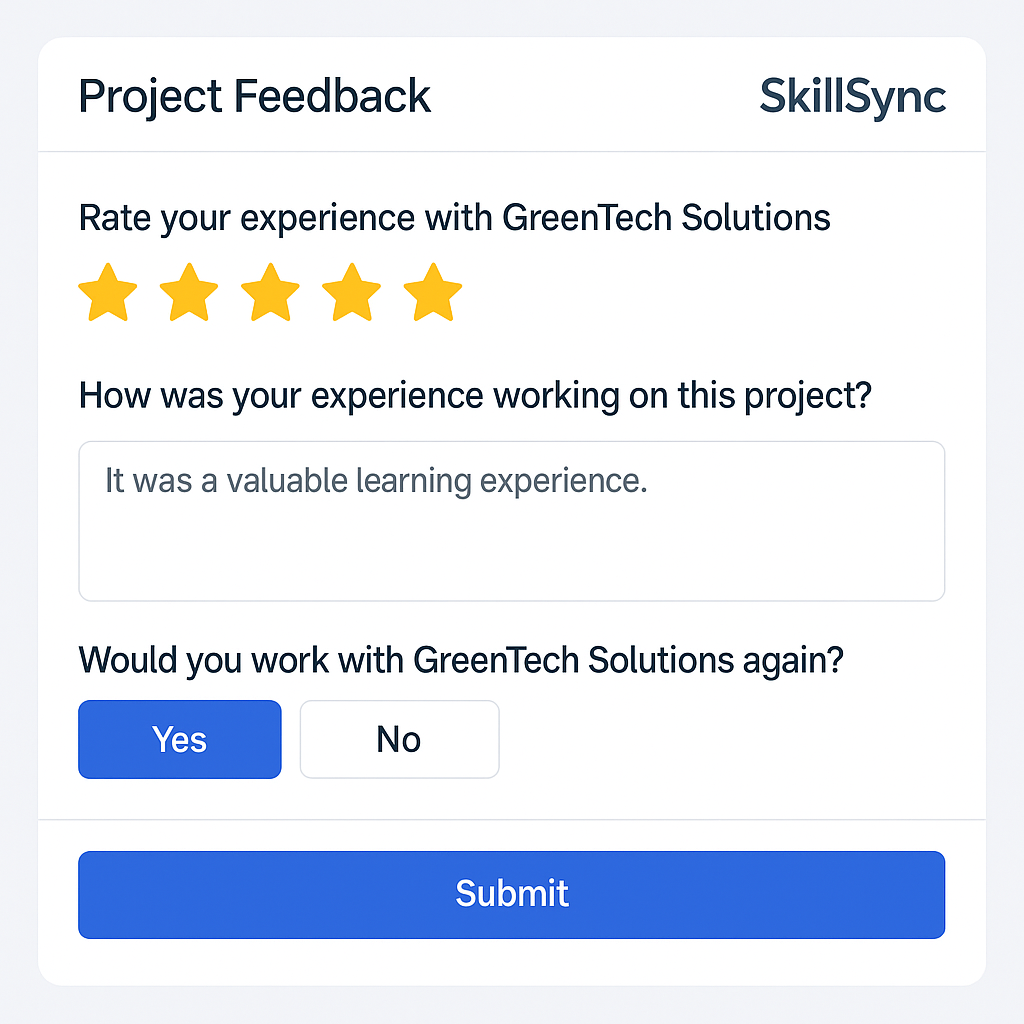
\includegraphics[width=0.8\linewidth]{figures/feedback-vurderingsskaerm.png}
  \caption{Feedback and evaluation screen (`feedback-vurderingsskaerm.png`) that powers the KPI loop.}
  \label{fig:feedback-screen}
\end{figure}

We built the analytics stack with reproducibility in mind. All dashboards include a ``definition'' tooltip that links to the dbt model and logic behind each metric. We version-control SQL queries, store key dashboards as code, and maintain a metrics catalogue so newcomers learn the context fast. Every quarter we archive snapshots of the KPI board so longitudinal analysis stays accurate even as definitions evolve. Those mundane habits are what turn metrics into institutional memory, aligning with \citet{Choudary2016}'s insistence that platforms must institutionalise learning, not just collect data.
